%%%%%%%%%%%%%%%%%%%%%%%%%%%%%%%%%%%%%%%%%%%%%%%%%%%%%%%%%%%%%%%%%%
%%%%%%%%%%%%%%%%%%%%%%%%%%%%%%%%%%%%%%%%%%%%%%%%%%%%%%%%%%%%%%%%%%
%Packages
\documentclass[10pt, a4paper]{article}
\usepackage[top=3cm, bottom=4cm, left=3.5cm, right=3.5cm]{geometry}
\usepackage{amsmath,amsthm,amsfonts,amssymb,amscd, fancyhdr, color, comment, graphicx, environ}
\usepackage{float}
\usepackage{mathrsfs}
\usepackage[math-style=ISO]{unicode-math}
\setmathfont{TeX Gyre Termes Math}
\usepackage{lastpage}
\usepackage{amsmath}
\usepackage[dvipsnames]{xcolor}
\usepackage[framemethod=TikZ]{mdframed}
\usepackage{enumerate}
\usepackage[shortlabels]{enumitem}
\usepackage{fancyhdr}
\usepackage{indentfirst}
\usepackage{listings}
\usepackage{sectsty}
\usepackage{thmtools}
\usepackage{shadethm}
\usepackage{hyperref}
\usepackage{setspace}
\usepackage{wrapfig}
\usepackage{ctex}
\usepackage{graphicx}%图片头文件
\usepackage{float} %指定图片位置
\usepackage{subfigure}%并排子图 共享标题 有子标题
\usepackage{caption}
\usepackage{fancyhdr}
\hypersetup{
    colorlinks=true,
    linkcolor=blue,
    filecolor=magenta,      
    urlcolor=blue,
}
%%%%%%%%%%%%%%%%%%%%%%%%%%%%%%%%%%%%%%%%%%%%%%%%%%%%%%%%%%%%%%%%%%
%%%%%%%%%%%%%%%%%%%%%%%%%%%%%%%%%%%%%%%%%%%%%%%%%%%%%%%%%%%%%%%%%%
%Environment setup
\mdfsetup{skipabove=\topskip,skipbelow=\topskip}
\newrobustcmd\ExampleText{%
An \textit{inhomogeneous linear} differential equation has the form
\begin{align}
L[v ] = f,
\end{align}
where $L$ is a linear differential operator, $v$ is the dependent
variable, and $f$ is a given non−zero function of the independent
variables alone.
}

\mdtheorem[style=theoremstyle]{Problem}{Problem}
\newenvironment{Solution}{\textbf{Solution.}}

%%%%%%%%%%%%%%%%%%%%%%%%%%%%%%%%%%%%%%%%%%%%%%%%%%%%%%%%%%%%%%%%%%
%%%%%%%%%%%%%%%%%%%%%%%%%%%%%%%%%%%%%%%%%%%%%%%%%%%%%%%%%%%%%%%%%%
%Fill in the appropriate information below
\newcommand{\norm}[1]{\left\lVert#1\right\rVert}     
\newcommand\course{Course}                      % <-- course name   
\newcommand\hwnumber{1}                         % <-- homework number
\newcommand\Information{XXX/xxxxxxxx}           % <-- personal information
%%%%%%%%%%%%%%%%%%%%%%%%%%%%%%%%%%%%%%%%%%%%%%%%%%%%%%%%%%%%%%%%%%
%%%%%%%%%%%%%%%%%%%%%%%%%%%%%%%%%%%%%%%%%%%%%%%%%%%%%%%%%%%%%%%%%%
%Page setup
\pagestyle{fancy}
\headheight 35pt
\lhead{SuZixin-12132416}
\lfoot{}
\pagenumbering{arabic}
\cfoot{\small\thepage}
\rfoot{}
\headsep 1.2em
\renewcommand{\baselinestretch}{1.25}       
\mdfdefinestyle{theoremstyle}{%
linecolor=black,linewidth=1pt,%
frametitlerule=true,%
frametitlebackgroundcolor=gray!20,
innertopmargin=\topskip,
}

%%%%%%%%%%%%%%%%%%%%%%%%%%%%%%%%%%%%%%%%%%%%%%%%%%%%%%%%%%%%%%%%%%
%%%%%%%%%%%%%%%%%%%%%%%%%%%%%%%%%%%%%%%%%%%%%%%%%%%%%%%%%%%%%%%%%%
%Add new commands here
\renewcommand{\labelenumi}{\alph{enumi})}
\newcommand{\Z}{\mathbb Z}
\newcommand{\R}{\mathbb R}
\newcommand{\Q}{\mathbb Q}
\newcommand{\NN}{\mathbb N}
\DeclareMathOperator{\Mod}{Mod} 
\renewcommand\lstlistingname{Algorithm}
\renewcommand\lstlistlistingname{Algorithms}
\def\lstlistingautorefname{Alg.}
%%%%%%%%%%%%%%%%%%%%%%%%%%%%%%%%%%%%%%%%%%%%%%%%%%%%%%%%%%%%%%%%%%
%%%%%%%%%%%%%%%%%%%%%%%%%%%%%%%%%%%%%%%%%%%%%%%%%%%%%%%%%%%%%%%%%%
%Begin now!



\begin{document}

\begin{titlepage}
    \begin{center}
        \vspace*{3cm}
            
        \Huge
        \textbf{HPC-FinalProject}
            
        \vspace{1cm}
        \huge
        Report
            
        \vspace{1.5cm}
        \Large
            
        \textbf{苏梓鑫-12132416}                      % <-- author
        
            
        \vfill
        
        
            
        \vspace{1cm}
            
        
\includegraphics[width=0.4\textwidth]{img/logo-sustech.png}
        \\
        
        \Large
        
        \today
            
    \end{center}
\end{titlepage}

%%%%%%%%%%%%%%%%%%%%%%%%%%%%%%%%%%%%%%%%%%%%%%%%%%%%%%%%%%%%%%%%%%
%%%%%%%%%%%%%%%%%%%%%%%%%%%%%%%%%%%%%%%%%%%%%%%%%%%%%%%%%%%%%%%%%%
%Start the assignment now

%%%%%%%%%%%%%%%%%%%%%%%%%%%%%%%%%%%%%%%%%%%%%%%%%%%%%%%%%%%%%%%%%%
%New problem
\clearpage  
\phantom{s}  
\thispagestyle{empty} 
\clearpage
\section{题目解析}
首先求出$\frac{\partial{u}}{\partial t}$ 的差分形式:
$$\frac{\partial u}{\partial t}=\frac{u(x,t_n+\Delta t)-u(x,t_n)}{\Delta t}=\frac{u^{n+1}_{i}-u^{n}_{i}}{\Delta t}$$
\subsection{显式求解}
$$u(x_i+\Delta x,t_n)=u(x_i,t_n)+\frac{\partial u}{\partial x}(x_i,t_n)\Delta x+\frac{\partial^2 u}{2\partial x^2}(x_i,t_n)\Delta x^2+O(\Delta x^3) $$
$$u(x_i-\Delta x,t_n)=u(x_i,t_n)-\frac{\partial u}{\partial x}(x_i,t_n)\Delta x+\frac{\partial^2 u}{2\partial x^2}(x_i,t_n)\Delta x^2+O(\Delta x^3)$$
两式相加得
$$\frac{\partial ^2u}{\partial x^2}=\frac{u(x_i+\Delta x,t_n)+u(x_i-\Delta x,t_n)-2u(x_i,t_n)}{\Delta x^2}=\frac{u_{i+i}^{n}+u_{i-1}^{n}-2u_{i}^{n}}{\Delta x^2}$$
代入:
$$\rho c\frac{\partial u}{\partial t}-k\frac{\partial ^2u}{\partial x^2}=f$$
有:
$$u_i^{n+1}=\frac{k\Delta t}{\rho c\Delta x^2}\left [
u^n_{i+1}+u^n_{i-1}+(\frac{\rho c\Delta x^2}{k\Delta t}-2)u_i^n
\right]+\frac{\Delta t}{\rho c}f^n_i$$
令
$$\lambda=\frac{k\Delta t}{\rho c\Delta x^2},\gamma=\frac{\Delta t}{\rho c}$$
则有:
$$u_i^{n+1}=
\lambda u^n_{i+1}+\lambda u^n_{i-1}+({1}-2\lambda)u_i^n
+\gamma f^n_i$$
将其写为矩阵形式:
$$u^{n+1}=Au^{n}+\gamma f^n$$
$$u^n=\begin{bmatrix}
u_1^n\\u^n_2\\.\\.\\u^n_N
\end{bmatrix}
f^n=\begin{bmatrix}
f_1^n\\f^n_2\\.\\.\\f^n_N
\end{bmatrix}
A=\begin{bmatrix}
1-2\lambda&\lambda&0&...&0\\
\lambda&1-2\lambda&\lambda&...&0\\
0&\lambda&1-2\lambda&...&0\\
...&...&...&&...\\
0&0&0&...&1-2\lambda
\end{bmatrix}$$
其中:
$$f=\sin(l\pi x),~~u_0=e^x,~~u(0,t)=u(1,t)=0,~~k=1.0$$
\subsection{隐式求解}
$$u(x_i+\Delta x,t_n+\Delta t)=u(x_i,t_n+\Delta t)+\frac{\partial u}{\partial x}(x_i,t_n+\Delta t)\Delta x+\frac{\partial^2 u}{2\partial x^2}(x_i,t_n+\Delta t)\Delta x^2+O(\Delta x^3)$$
$$u(x_i-\Delta x,t_n+\Delta t)=u(x_i,t_n+\Delta t)-\frac{\partial u}{\partial x}(x_i,t_n+\Delta t)\Delta x+\frac{\partial^2 u}{2\partial x^2}(x_i,t_n+\Delta t)\Delta x^2+O(\Delta x^3)$$
两式相加得
$$
\frac{\partial ^2u}{\partial x^2}=\frac{u(x_i+\Delta x,t_n+\Delta t)+u(x_i-\Delta x,t_n+\Delta t)-2u(x_i,t_n+\Delta t)}{\Delta x^2}\\
=\frac{u_{i+i}^{n+1}+u_{i-1}^{n+1}-2u_{i}^{n+1}}{\Delta x^2}$$
代入:
$$
\rho c\frac{\partial u}{\partial t}-k\frac{\partial ^2u}{\partial x^2}=f
$$
有:
$$
u_i^{n+1}=\frac{k\Delta t}{\rho c\Delta x^2}\left [
u^{n+1}_{i+1}+u^{n+1}_{i-1}-2u_i^{n+1}
\right]+\frac{\Delta t}{\rho c}f^n_i+u_i^n
$$
有:
$$
u^n_i+\gamma f_i^n=\lambda \left[
(2+\frac{1}{\lambda})u_i^{n+1}-u^{n+1}_{i+1}-u^{n+1}_{i-1}
\right]
$$
将其写为矩阵形式:
$$
u^{n}+\gamma f^n=Au^{n+1}
$$
$$
u^n=\begin{bmatrix}
u_1^n\\u^n_2\\.\\.\\u^n_N
\end{bmatrix}
f^n=\begin{bmatrix}
f_1^n\\f^n_2\\.\\.\\f^n_N
\end{bmatrix}
A=\begin{bmatrix}
1+2\lambda&-\lambda&0&...&0\\
-\lambda&1+2\lambda&-\lambda&...&0\\
0&-\lambda&1+2\lambda&...&0\\
...&...&...&&...\\
0&0&0&...&1+2\lambda
\end{bmatrix}
$$
其中:
$$
f=\sin(l\pi x),~~u_0=e^x,~~u(0,t)=u(1,t)=0,~~k=1.0
$$
\subsection{解析解}
已知$\rho=1.0,c=1.0,k=1.0$,且$f=\sin(l\pi x)$,$u(0,t)=u(1,t)=0$ 
因为当边界和初始数据与时间无关时,偏微分方程的解将随着时间t收敛到稳态解,因此有:
$$
\frac{\partial u}{\partial t}=0
$$
$$
\rho c\frac{\partial u}{\partial t}-k\frac{\partial ^2u}{\partial x^2}=f ~~\rightarrow ~~\frac{\partial ^2u}{\partial x^2}=-\sin(l\pi x)
$$
两边同时对x积分得:
$$
\frac{\partial u}{\partial x}=\frac{cos(l\pi x)}{l\pi}+C_1
$$
两边同时再对x 积分得:
$$
u=\frac{\sin(l\pi x)}{l^2\pi ^2}+C_1x+C_2
$$
代入边界条件$u(0,t)=u(1,t)=0$:
$$
u=\frac{\sin(l\pi x)}{l^2\pi ^2}-\frac{\sin(l\pi)}{l^2\pi ^2}x
$$
\clearpage
\section{程序实现}
这一部分大致讲解一下如何采用Petsc 实现两种迭代形式,以及如何添加重启功能和防御性编程写法,程序流程比较简单,因此具体细节不多赘述。
三个功能的程序流程图如下所示:

\begin{figure}[H]
\centering
\subfigure[显式迭代程序流程图.]{
\begin{minipage}[t]{0.3\linewidth}
\centering
\includegraphics[scale=0.35]{img/proc-显式迭代.png}
%\caption{fig1}
\end{minipage}%
}%
\subfigure[隐式迭代程序流程图.]{
\begin{minipage}[t]{0.3\linewidth}
\centering
\includegraphics[scale=0.35]{img/proc-隐式迭代.png}
%\caption{fig2}
\end{minipage}%
}%
\subfigure[重启功能程序流程图.]{
\begin{minipage}[t]{0.3\linewidth}
\centering
\includegraphics[scale=0.35]{img/proc-重读流程图.png}
%\caption{fig3}
\end{minipage}%
}%
\centering
\caption{ 总体程序流程图}
\end{figure}
\subsection{显式求解}
显式求解的形式在1中已经说明,采用矩阵形式迭代,我们
需要组装一个矩阵A,以及需要若干向量辅助。需要一个f,还
有两个u,一个u-now,一个u-last,用于迭代。最后结果为
u-now。程序流程图如图1-(a)所示。
使用了Petsc 的MatMultAdd函数进行计算,这个函数的作用是求$u_{now}=Au_{last}+f$。
~\\

MatMultAdd(A, u-last, f, u-now);


\subsection{隐式求解}
隐式求解相比显示求解来说多了一些步骤,需要添加ksp进行求解。其用到的
变量基本与显示求解的相同,这里不再解释。程序流程图如图1-(b)所示。
使用了Petsc的VecWAXPY 和 KSPSolve 两个函数,功能是求 $b=f+u_{last}$ 
以及解线性方程组,$u_{now}=Ab$
~\\

VecWAXPY(b, 1.0, f, u-last);
KSPSolve(ksp, b, u-now);



\subsection{重启功能}
重启功能主要利用Petsc 中的HDF5 功能,首先利用PetscViewerHDF5Open(),创建HDF5文件并打开。
在迭代过程中每10步进行一次写入,判断 $ (!it\%10)==1 $
是否成立。存储的变量有:
\begin{enumerate}
    \item 对x划分大小 size
    \item 时间步大小 dt
    \item 迭代次数 it
\end{enumerate}
把这三个变量存储在temp 向量里,并且起了别名叫做:xxplicit-temp。利用VecView 写入HDF5 文件中。
接着把$u_{now}$ 保存到文件里,最后需要进行析构viewer。
重启功能的程序流程图如图1-(c) 所示。
\subsection{防御性编程}
除了注释和变量名之外,增加了

断言:监测下面三个量:$dx, iteration_{num}, gamma$不能=0

\begin{figure}[!h]
%是可选项 h表示的是here在这里插入,t表示的是在页面的顶部插入
\centering
\includegraphics[scale=0.6]{img/Assert.png}
\caption{Assert Code.}
\label{fig:1}
\end{figure}

处理异常
:在CFL>0.5的情况下,程序无法收敛,为了防止计算资源浪费,直接跳出程序。
\begin{figure}[!h]
%是可选项 h表示的是here在这里插入,t表示的是在页面的顶部插入
\centering
\includegraphics[scale=0.4]{img/CFL.png}
\caption{判断是否收敛.}
\label{fig:1}
\end{figure}

\clearpage
\section{性能分析}
\subsection{Valgrind}
\subsubsection{内存检测}
采用valgrind 对内存进行检测,执行:valgrind ./exec 然后查看结果如下:
\begin{figure}[!h]
%是可选项 h表示的是here在这里插入,t表示的是在页面的顶部插入
\centering
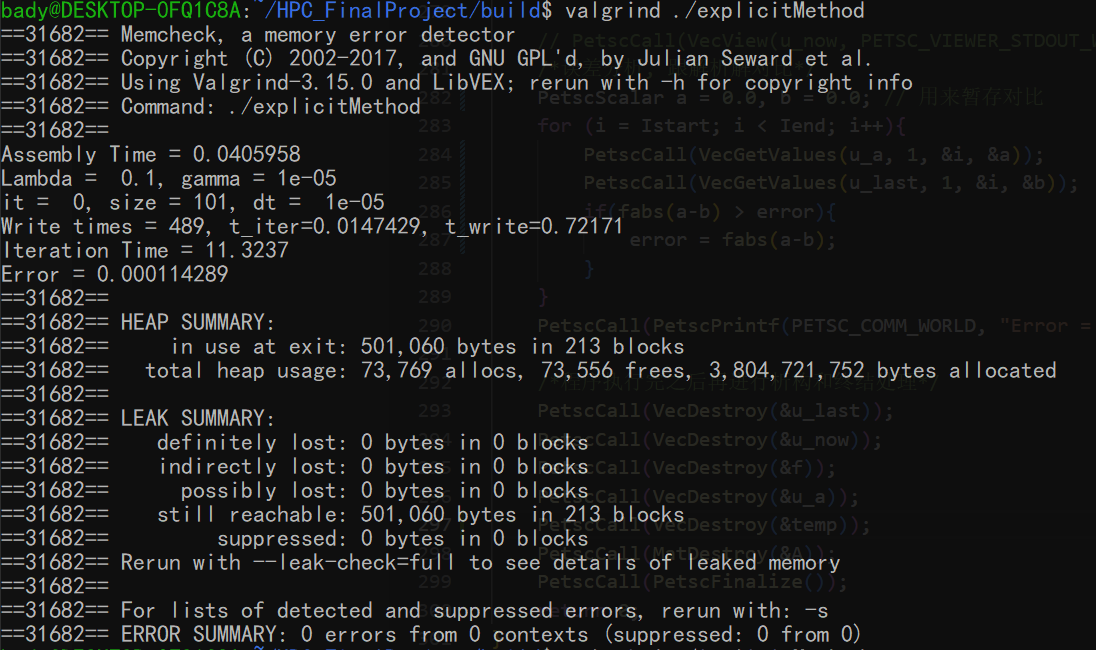
\includegraphics[scale=0.3]{img/Valgrind-pre.png}
\caption{Valgrind 改进前的显式程序}
\label{fig:1}
\end{figure}
\begin{figure}[!h]
%是可选项 h表示的是here在这里插入,t表示的是在页面的顶部插入
\centering
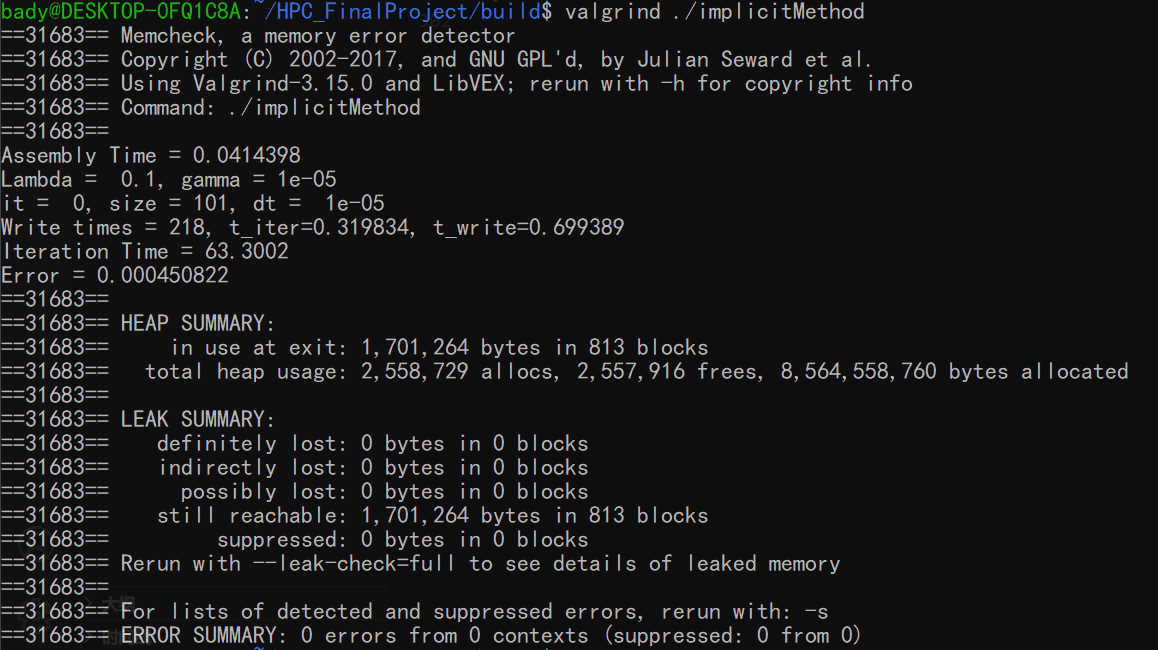
\includegraphics[scale=0.3]{img/Valgrind-pre2.png}
\caption{Valgrind 改进前的隐式程序}
\label{fig:1}
\end{figure}
我们可以看出出现了一些 still reachable的错误,泄露的量有1000个blocks,
这说明在程序结束之后还有一些变量还被程序占用着,但是过一段时间会自动释放。
在section 3.2 中会对这个问题进行解决。
\subsubsection{性能检测}
采用指令:valgrind --tool=callgrind ./exec 得到得结果如下:

\begin{figure}[!h]
%是可选项 h表示的是here在这里插入,t表示的是在页面的顶部插入
\centering
\includegraphics[scale=0.3]{img/Valgrind-file.png}
\caption{Valgrind 得到的文件}
\label{fig:1}
\end{figure}

对程序运行的时间进行检测,采用qcachegrind 查看程序情况如下:

显式:
\begin{figure}[!h]
%是可选项 h表示的是here在这里插入,t表示的是在页面的顶部插入
\centering
\includegraphics[scale=0.35]{img/Callgrind-显式1.png}
\caption{Callgrind 显式运行时间}
\label{fig:1}
\end{figure}
\begin{figure}[!h]
%是可选项 h表示的是here在这里插入,t表示的是在页面的顶部插入
\centering
\includegraphics[scale=0.4]{img/Callgrind-显式2.png}
\caption{Callgrind 显式Main函数时间分布图}
\label{fig:1}
\end{figure}
\begin{figure}[!h]
%是可选项 h表示的是here在这里插入,t表示的是在页面的顶部插入
\centering
\includegraphics[scale=0.4]{img/Callgrind-显式3.png}
\caption{Callgrind 显式函数调用}
\label{fig:1}
\end{figure}

从图7--图9,我们可以看出总体的分布就是MatMultAdd 这个函数占据了大部分的运行时间
性能的瓶颈在这里,提升这部分性能可以提高程序的效率。

隐式:

\begin{figure}[!h]
%是可选项 h表示的是here在这里插入,t表示的是在页面的顶部插入
\centering
\includegraphics[scale=0.35]{img/Callgrind-隐式1.png}
\caption{Callgrind 隐式运行时间}
\label{fig:1}
\end{figure}
\begin{figure}[!h]
%是可选项 h表示的是here在这里插入,t表示的是在页面的顶部插入
\centering
\includegraphics[scale=0.4]{img/Callgrind-隐式2.png}
\caption{Callgrind 隐式Main函数时间分布图}
\label{fig:1}
\end{figure}
\begin{figure}[!h]
%是可选项 h表示的是here在这里插入,t表示的是在页面的顶部插入
\centering
\includegraphics[scale=0.4]{img/Callgrind-隐式3.png}
\caption{Callgrind 隐式函数调用}
\label{fig:1}
\end{figure}
从图10--图12,我们可以看出在隐式求解中,KSPSolve占据了87\%以上的时间,主要是因为求解线性方程组消耗大。
即 KSPSolve是程序的瓶颈,这部分的改进将会大幅度加速程序的运行,在后面测试环节加入预处理子进行测试。


\subsection{改进}
3.1中出现了内存泄漏问题,这里一并解决,存在的内存泄露问题来自下面这个代码,在写入的时候频繁创建打开,但是实际上并不需要。将PetscViewerCreate,删除。并且把PetscViewerHDF5Open 移到循环外。还有一个问题是忘记把ksp析构了。

\begin{figure}[!h]
%是可选项 h表示的是here在这里插入,t表示的是在页面的顶部插入
\centering
\includegraphics[scale=0.5]{img/Leak.png}
\caption{内存泄漏主要代码}
\label{fig:1}
\end{figure}

重新检测之后得到如下,此时的内存泄漏为0,可以看出内存泄漏问题解决了。

\begin{figure}[!h]
%是可选项 h表示的是here在这里插入,t表示的是在页面的顶部插入
\centering
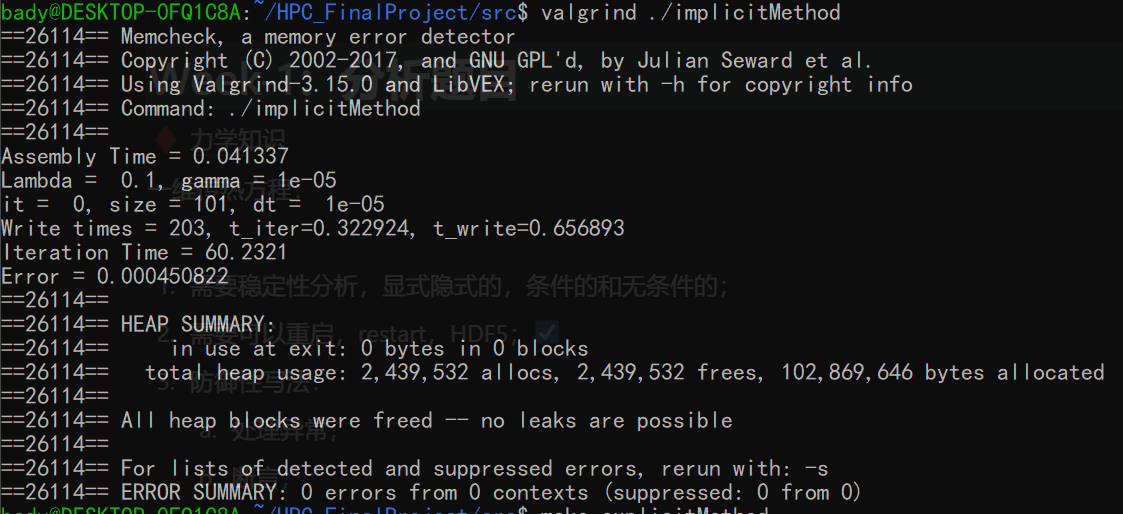
\includegraphics[scale=0.33]{img/Valgrind-after.png}
\caption{Valgrind 改进后显式程序}
\label{fig:1}
\end{figure}
\begin{figure}[!h]
%是可选项 h表示的是here在这里插入,t表示的是在页面的顶部插入
\centering
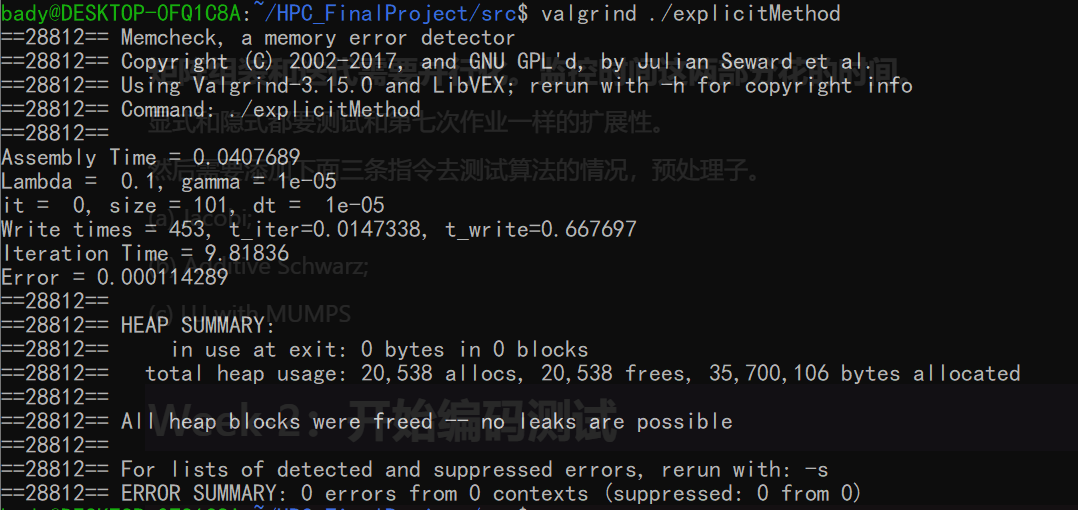
\includegraphics[scale=0.35]{img/Valgrind-after2.png}
\caption{Valgrind 改进后隐式程序}
\label{fig:1}
\end{figure}


\clearpage
\section{测试}
测试部分有六个模块,整体划分为两个部分。

第一个部分:正确性,稳定性,这部分内容需要的计算规模比较小,因此这一部分主要在本地机器进行测试。

第二个部分:误差分析,并行性分析和预处理子测试,这部分需要的计算规模较大,所以这部分采用TAIYI进行结果测试。因为数量众多,这里只取部分结果进行绘图展示。
\subsection{正确性}
正确性测试的测试参数为:-size 100 -dt 0.00001 , 与程序中计算出来的精确解结果进行对比。
精确解在第1部分已经分析过。

画图使用python,源代码位于github仓库的report文件夹内。
\subsubsection{显式迭代}
\begin{figure}[H]
\centering
\subfigure[放大结果.]{
\begin{minipage}[t]{0.4\linewidth}
\centering
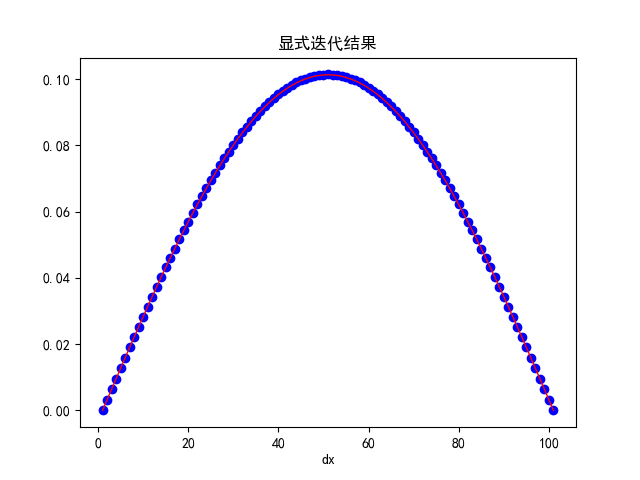
\includegraphics[scale=0.35]{img/显式结果.png}
%\caption{fig1}
\end{minipage}%
}%
\subfigure[总体结果.]{
\begin{minipage}[t]{0.4\linewidth}
\centering
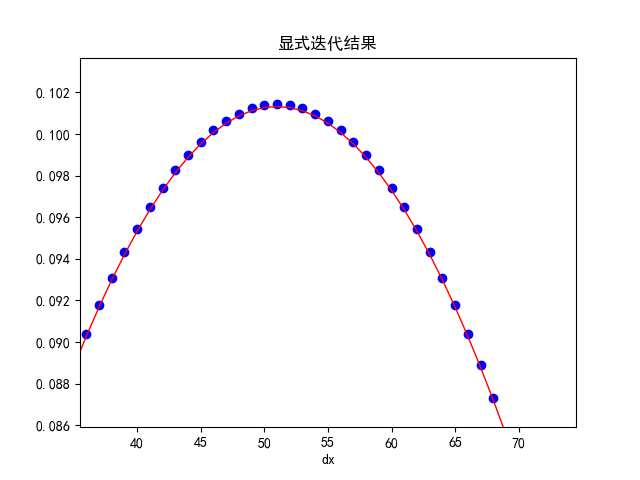
\includegraphics[scale=0.35]{img/显式放大.png}
%\caption{fig2}
\end{minipage}%
}%
\centering
\caption{ 显式正确性测试结果}
\end{figure}

对比之后发现结果相近,证明显式迭代是正确的,误差为:9.827e-5可以认为误差较小。

\subsubsection{隐式迭代}

\begin{figure}[H]
\centering
\subfigure[放大结果.]{
\begin{minipage}[t]{0.4\linewidth}
\centering
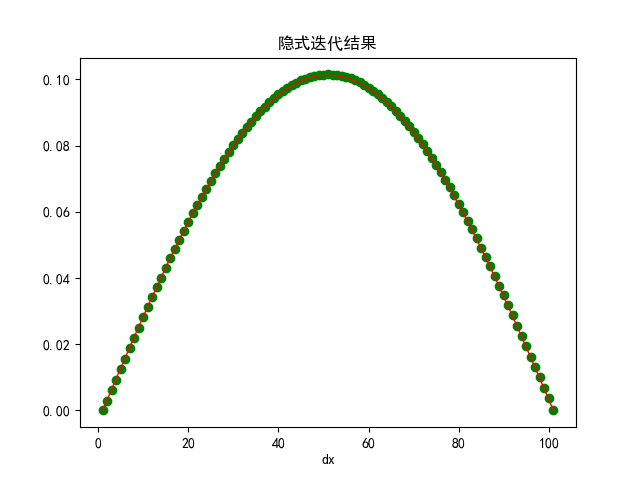
\includegraphics[scale=0.35]{img/隐式结果.png}
%\caption{fig1}
\end{minipage}%
}%
\subfigure[总体结果.]{
\begin{minipage}[t]{0.4\linewidth}
\centering
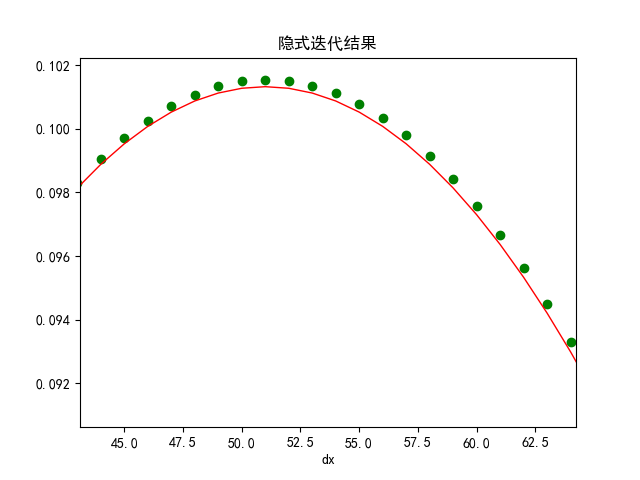
\includegraphics[scale=0.35]{img/隐式放大.png}
%\caption{fig2}
\end{minipage}%
}%
\centering
\caption{ 显式正确性测试结果}
\end{figure}

对比之后发现结果相近,证明隐式迭代是正确的,误差为:4.231e-4可以认为误差较小。

\subsubsection{重启功能}
在程序运行中用ctrl + c 打断程序,然后用下面指令查看结果

/home/bady/lib/hdf5/bin/h5dump implicitMethod.h5

\begin{figure}[!h]
%是可选项 h表示的是here在这里插入,t表示的是在页面的顶部插入
\centering
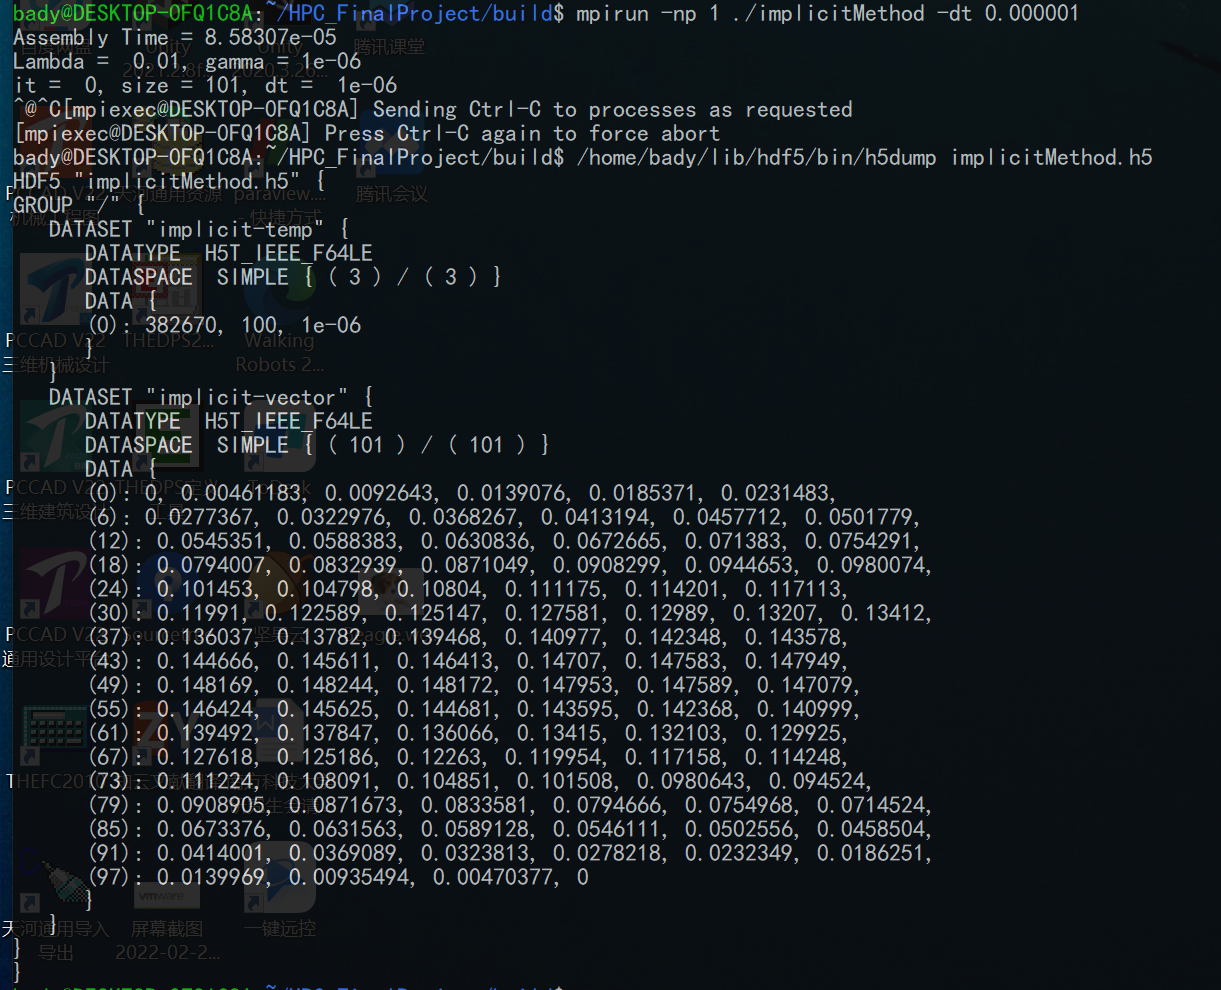
\includegraphics[scale=0.3]{img/restart1.png}
\caption{HDF5 结果}
\label{fig:1}
\end{figure}

然后启动 -restart 1,重新启动,最后得到的结果如下:和隐式迭代的结果对比。

\begin{figure}[!h]
%是可选项 h表示的是here在这里插入,t表示的是在页面的顶部插入
\centering
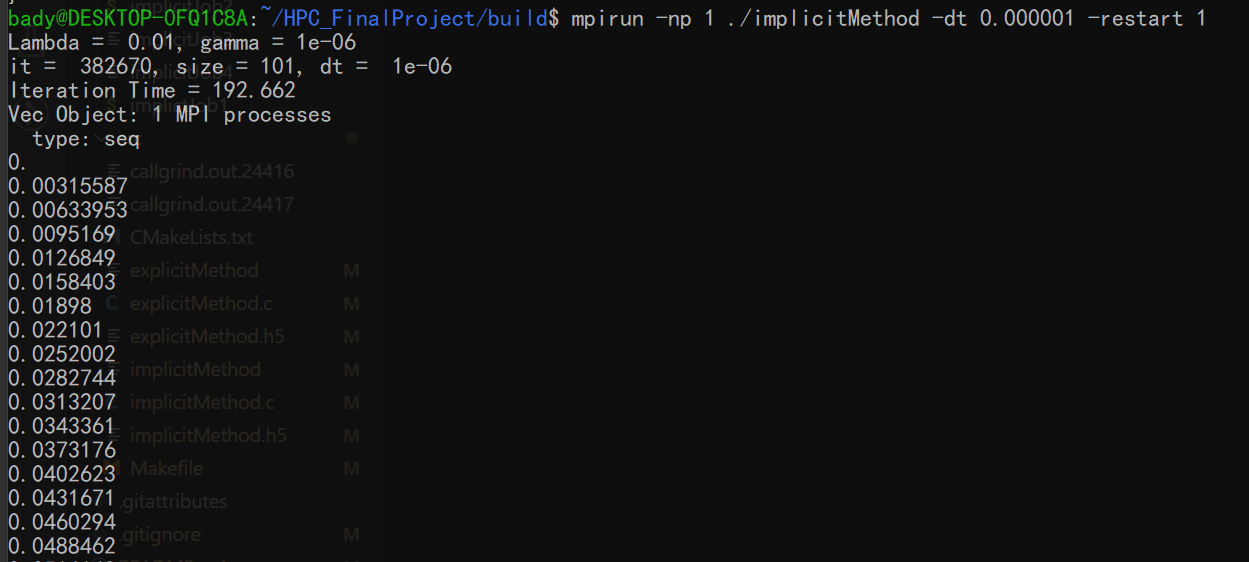
\includegraphics[scale=0.3]{img/restart2.png}
\caption{重启计算结果}
\label{fig:1}
\end{figure}

可以看到前面几行结果都吻合,注意这里的it就是被打断位置上的迭代步数,同时没有显示Assembly Time说明没有进行向量设置。

\begin{figure}[!h]
%是可选项 h表示的是here在这里插入,t表示的是在页面的顶部插入
\centering
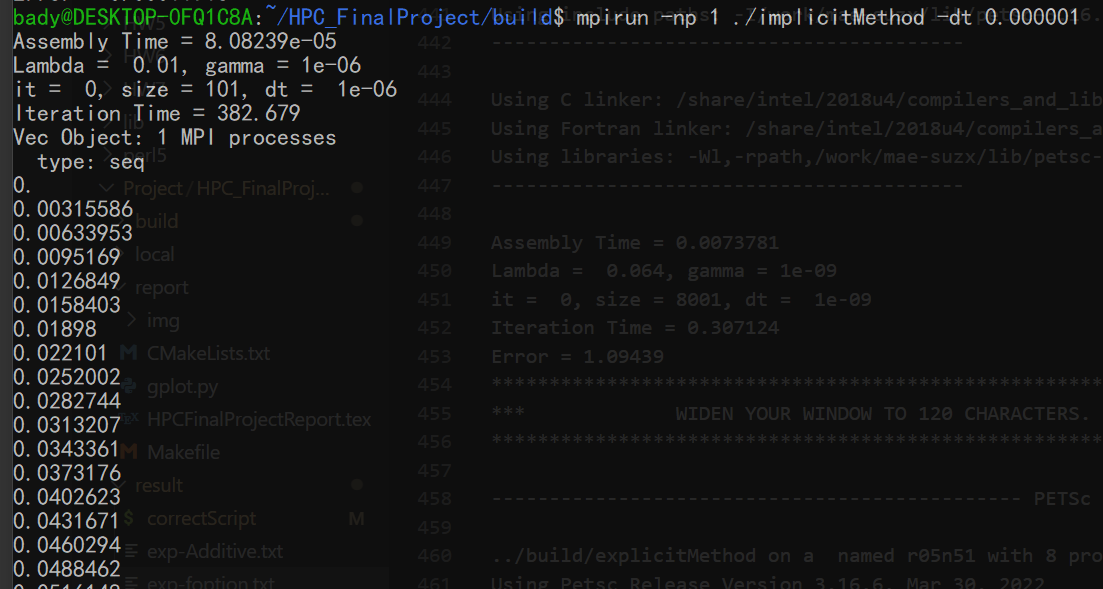
\includegraphics[scale=0.3]{img/restart3.png}
\caption{正常运行计算结果}
\label{fig:1}
\end{figure}

\subsection{组装矩阵和向量的并行}
改进前:for (i = 0; i < size+1; i++)

直接采用从0设置到size+1,这样会让计算机从0开始运行,从而无法并行,因为下个processor需要知道上一个跑到哪里。

\begin{figure}[!h]
%是可选项 h表示的是here在这里插入,t表示的是在页面的顶部插入
\centering
\includegraphics[scale=0.5]{img/组装对比1.png}
\caption{改进前组装结果}
\label{fig:1}
\end{figure}

改进后,从每个核处理的第一个数据到最后一个数据,这样提高了并行性。

    VecGetOwnershipRange($u_last$, Istart, Iend);
    
    for (i = Istart; i < Iend; i++)

从图21和图22两幅图我们可以看出,相比于不分块组装矩阵或向量,分块的速度要更快,运行时间较短,核数增加其提高的效率也随着增加。在单核情况下两个部分的组装时间相似,没有特别大的差异。

\begin{figure}[!h]
%是可选项 h表示的是here在这里插入,t表示的是在页面的顶部插入
\centering
\includegraphics[scale=0.5]{img/组装对比2.png}
\caption{改进后组装结果}
\label{fig:1}
\end{figure}

\subsection{稳定性分析}
\subsubsection{显式迭代}
由1 知道,

$$
u_i^{n+1}=
\lambda u^n_{i+1}+\lambda u^n_{i-1}+({1}-2\lambda)u_i^n
+\gamma f^n_i
$$

最坏的情况即,增长系数$G=1-2\lambda-\lambda-\lambda =1-4\lambda$ 

令$|G|<1=> ~~即|1-4\lambda|<1$ 解得:

$$
\lambda\le 0.5
$$

实际测试如下,可以看到size=10时,需要dt<=0.005 才能收敛。

\begin{figure}[H]
\centering
\subfigure[显示稳定性耗时1.]{
\begin{minipage}[t]{0.4\linewidth}
\centering
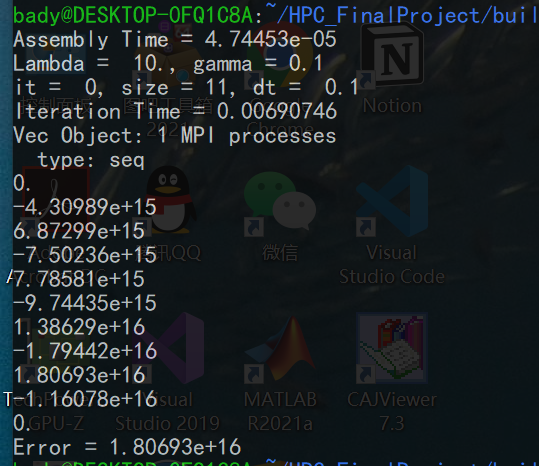
\includegraphics[scale=0.4]{img/显式稳定性1.png}
%\caption{fig1}
\end{minipage}%
}%
\subfigure[显示稳定性耗时2.]{
\begin{minipage}[t]{0.4\linewidth}
\centering
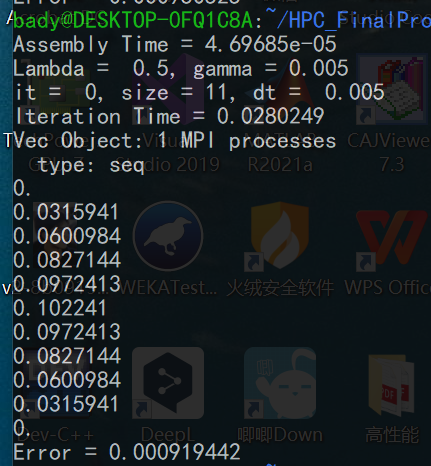
\includegraphics[scale=0.4]{img/显式稳定性2.png}
%\caption{fig2}
\end{minipage}%
}%
\centering
\caption{ 显示稳定性耗时}
\end{figure}


\subsubsection{隐式迭代}
隐式迭代是无条件收敛的,因为其增长因子在所有情况下都符合<1;
$G=\frac{1}{1+4\lambda sin^2(\Delta x)}$,其中$\lambda sin^2(\Delta x)>0$
因此$|G|<1$,所以无论$\Delta t$取多大隐式迭代都能收敛。

实际测试如下,可以看到size=10时,dt 取任何值都能收敛,但是计算效率低,耗时相比显示的更高。



\begin{figure}[!h]
%是可选项 h表示的是here在这里插入,t表示的是在页面的顶部插入
\centering
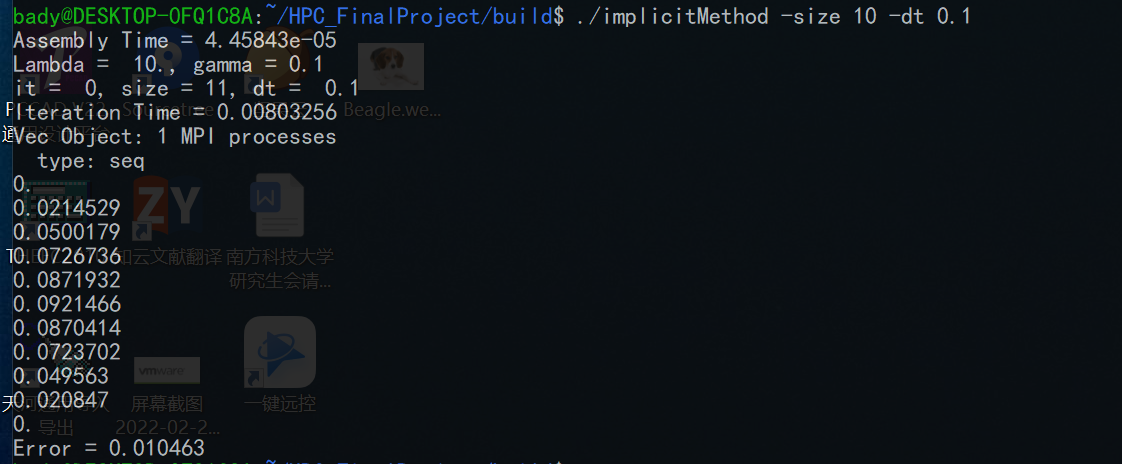
\includegraphics[scale=0.3]{img/隐式稳定性1.png}
\caption{隐式稳定性耗时1}
\label{fig:1}
\end{figure}

\begin{figure}[!h]
%是可选项 h表示的是here在这里插入,t表示的是在页面的顶部插入
\centering
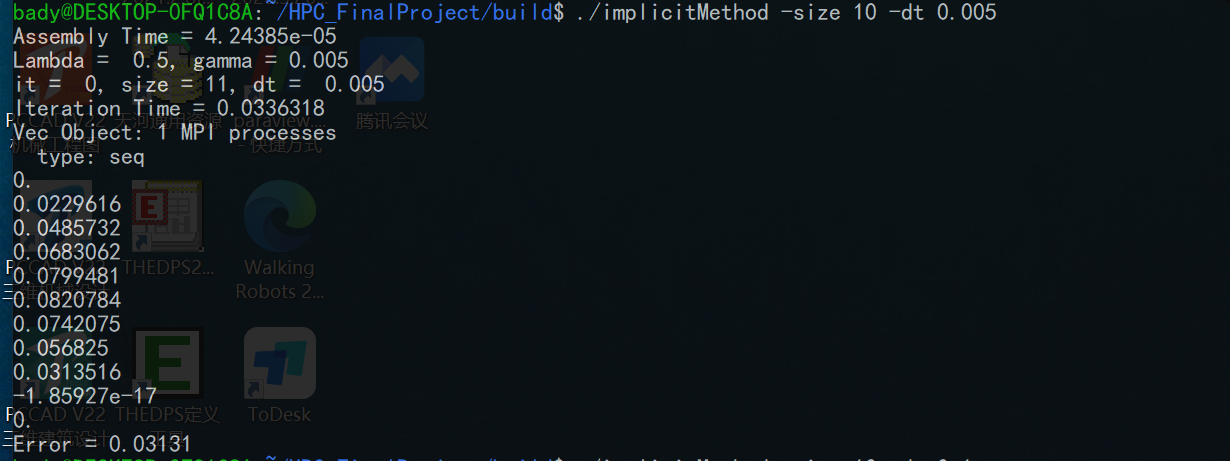
\includegraphics[scale=0.3]{img/隐式稳定性2.png}
\caption{隐式稳定性耗时2}
\label{fig:1}
\end{figure}

\subsubsection{收敛时间速度对比}
取误差为0.01,size=400,最快达到误差范围内的迭代次数和迭代时间如下:

\begin{figure}[H]
\centering
\subfigure[显示收敛速度.]{
\begin{minipage}[t]{0.5\linewidth}
\centering
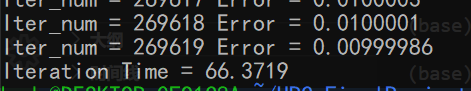
\includegraphics[scale=0.4]{img/显式收敛速度.png}
%\caption{fig1}
\end{minipage}%
}%
\subfigure[隐式收敛速度.]{
\begin{minipage}[t]{0.5\linewidth}
\centering
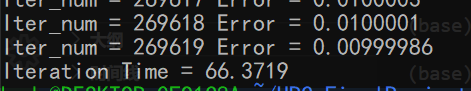
\includegraphics[scale=0.4]{img/显式收敛速度.png}
%\caption{fig2}
\end{minipage}%
}%
\centering
\caption{ 收敛速度对比}
\end{figure}

因此我们可以看出收敛速度和迭代时间均是显式更好,但是显式是条件稳定的在矩阵越大时需要的计算步数会更多。

\subsection{误差分析}
取size = 50, 60, 70, 80, 90, 100, dt=0.000005 进行测试:
得到结果如下图所示

\begin{figure}[!h]
%是可选项 h表示的是here在这里插入,t表示的是在页面的顶部插入
\centering
\includegraphics[scale=0.8]{img/error.png}
\caption{误差分析图}
\label{fig:1}
\end{figure}

经过计算大致,$\frac{log(error)}{log(dx)}=2$

\subsection{并行性}
\subsubsection{显式迭代}
固定矩阵大小为  10000

~\\

\begin{tabular}{|c|c|c|c|c|c|c|c|c|c|c|}% 通过添加 | 来表示是否需要绘制竖线
\hline  % 在表格最上方绘制横线
核数&1&2&3&4&5&6&7&8&9\\
\hline  %在第一行和第二行之间绘制横线
时间&1.6489&1.2659&1.07849&1.0285&1.1265&1.241&1.2488&1.3419&1.5128\\
\hline % 在表格最下方绘制横线
\end{tabular}

~\\

从上表我们可以看出,运行时间先减少后增加这是因为,一开始矩阵比较大分块比较合适,而当超过一定阈值之后矩阵大小已经达到最优不需要再分了,此时分解反而导致结果更慢。

固定计算量$GFLop = 3.0\times 10^8$不变,增加核数

~\\

\begin{tabular}{|c|c|c|c|c|c|c|c|}% 通过添加 | 来表示是否需要绘制竖线
\hline  % 在表格最上方绘制横线
核数&4&5&6&7&8&9\\
\hline  %在第一行和第二行之间绘制横线
时间&0.79891&0.95509&1.0838&1.2052&1.3297&1.4989\\
\hline % 在表格最下方绘制横线
\end{tabular}

~\\

从上表我们可以看出当核数增加时时间也增加,但是是近似于等差的增加,因为增加了相同的工作量,但是后面核数增加之后时间增加的越来越小是因为矩阵大小变得比较大此时并行的效率高。

后续规律基本与这里相同后面只罗列出数据,不再重复。

\subsubsection{隐式迭代}

~\\

\begin{tabular}{|c|c|c|c|c|c|c|c|c|}% 通过添加 | 来表示是否需要绘制竖线
\hline  % 在表格最上方绘制横线
核数&3&4&5&6&7&8&9\\
\hline  %在第一行和第二行之间绘制横线
时间&1.12746&1.0178&0.820482&0.735693&0.910889&0.872818&0.713241\\
\hline % 在表格最下方绘制横线
\end{tabular}

~\\

~\\



\begin{tabular}{|c|c|c|c|c|c|c|c|c|}% 通过添加 | 来表示是否需要绘制竖线
\hline  % 在表格最上方绘制横线
核数&3&4&5&6&7&8&9\\
\hline  %在第一行和第二行之间绘制横线
时间&0.552447&0.672541&0.85896&0.987344&1.129162&1.382166&1.538699\\
\hline % 在表格最下方绘制横线
\end{tabular}

~\\



\subsection{预处理子}

这里只对显式程序进行测试,我们可以看到这里的结果都不是很理想,比起没有加预处理子的结果并没有多大的提升,我猜测
的原因是:计算规模太小,因为这里只是测试一下并行性,所以我没有让程序有很大的规模,而是跑到一定的迭代次数就停止了。
因此可能会有一些计算量上的差异,以及可能存在的偶然性,导致最后出现的结果不理想。

--Jacobi

~\\

\begin{tabular}{|c|c|c|c|c|c|c|c|c|c|c|}% 通过添加 | 来表示是否需要绘制竖线
\hline  % 在表格最上方绘制横线
核数&1&2&3&4&5&6&7&8&9\\
\hline  %在第一行和第二行之间绘制横线
时间&1.6833&1.2647&1.0729&1.0306&1.1618&1.2464&1.2665&1.3439&1.5115\\
\hline % 在表格最下方绘制横线
\end{tabular}

~\\

~\\

\begin{tabular}{|c|c|c|c|c|c|c|c|c|c|c|}% 通过添加 | 来表示是否需要绘制竖线
\hline  % 在表格最上方绘制横线
核数&4&5&6&7&8&9\\
\hline  %在第一行和第二行之间绘制横线
时间&0.780179&0.937723&1.07553&1.20361&1.3297&1.54505\\
\hline % 在表格最下方绘制横线
\end{tabular}

~\\

--Additive 

~\\

\begin{tabular}{|c|c|c|c|c|c|c|c|c|c|c|}% 通过添加 | 来表示是否需要绘制竖线
\hline  % 在表格最上方绘制横线
核数&1&2&3&4&5&6&7&8&9\\
\hline  %在第一行和第二行之间绘制横线
时间&1.7478&1.2564&1.0966&1.0357&1.1665&1.25391&1.2644&1.3679&1.5862\\
\hline % 在表格最下方绘制横线
\end{tabular}

~\\

\begin{tabular}{|c|c|c|c|c|c|c|c|c|}% 通过添加 | 来表示是否需要绘制竖线
\hline  % 在表格最上方绘制横线
核数&4&5&6&7&8&9\\
\hline  %在第一行和第二行之间绘制横线
时间&0.791735&0.949634&1.07991&1.19482&1.34177&1.50548\\
\hline % 在表格最下方绘制横线
\end{tabular}

~\\



--MUMPS

~\\

\begin{tabular}{|c|c|c|c|c|c|c|c|c|c|c|}% 通过添加 | 来表示是否需要绘制竖线
\hline  % 在表格最上方绘制横线
核数&1&2&3&4&5&6&7&8&9\\
\hline  %在第一行和第二行之间绘制横线
时间&1.6455&1.2679&1.0851&1.0377&1.1271&1.2372&1.2524&1.3875&1.5427\\
\hline % 在表格最下方绘制横线
\end{tabular}

~\\

~\\

\begin{tabular}{|c|c|c|c|c|c|c|c|}% 通过添加 | 来表示是否需要绘制竖线
\hline  % 在表格最上方绘制横线
核数&4&5&6&7&8&9\\
\hline  %在第一行和第二行之间绘制横线
时间&0.788799&0.940163&1.086&1.22918&1.31874&1.53477\\
\hline % 在表格最下方绘制横线
\end{tabular}

~\\


\clearpage
\section*{Appendix}

没时间写了

一些改动之后又改回来的东西:

耗时最多是HDF5 的存储功能,原本是每10次迭代存储一次,因为实际测试是迭代速度很快,每10次存储的开销太大了,因此测试了一次迭代所花的时间$T_{iter}$,和一次写数据所花的时间$T_{write}$。计算$n=\frac{T_{write}}{T_{iter}}$,取整,作为10*n次迭代存储一次数据。

改进部分的代码如下,得到的$n_step,n_step$保存一次结果:
%%%%%%%%%%%%%%%%%%%%%%%%%%%%%%%%%%%%%%%%%%%%%%%%%%%%%%%%%%%%%%%%%%
%Complete the assignment now
\end{document}

%%%%%%%%%%%%%%%%%%%%%%%%%%%%%%%%%%%%%%%%%%%%%%%%%%%%%%%%%%%%%%%%%%
%%%%%%%%%%%%%%%%%%%%%%%%%%%%%%%%%%%%%%%%%%%%%%%%%%%%%%%%%%%%%%%%%%
